\chapter{Использование сверточных нейронных сетей в задаче распознавания изображений}

\section{Сверточные нейронные сети}
\subsection{Проблема распознавания изображений}
При использовании полносвязной нейронной сети для распознавания сложных, цветных изображений выявляется ряд сложностей. Первая проблема --- плохая прооизводительность алгоритма при работе с большими векторами признаков: для цветного растрового изображения в разрешении $200 \times 200$ необходимо будет составлять вектор признаков из тензора размерностью $200 \times 200 \times 3$, первый слой полносвязной сети должен состоять из $120000$ нейронов, что очень сильно сказывается на потребляемых ресурсах. Вторая проблема --- малая эффективность в обучении: нейронная сеть не берет во внимание геометрию и взаимное расположение объектов, вместо этого она работает лишь с конкретными пикселями. Это сильно сказывается на качестве обучения \cite{20}.
\subsection{Понятие свертки изображений}
Для решения данных проблем необходимо было создавать на основе изображения более корректный вектор признаков, который бы в себе учитывал геометрию и взаимное расположение объектов на изображении, так же он должен быть достаточно маленькой размерности, чтобы обучение было эффективным по времени. Такая подготовка изображения опирается на понятие свертки. Свертка в машинном обучении --- поэлементное перемножение матрицы изображения и матрицы ядра(фильтра) и суммирование элементов с целью получить новую матрицу путем сдвига по длине и ширине, для многоканального изображения для каждого канала используется свое ядро и значения матриц суммируются. Ядро(фильтр) --- квадратная матрица состоящая из параметров, которые нужно получить в ходе обучения. Полученные в ходе свертки данные явлются картой признаков. Она показывает области наибольшей активации ядра.

Процесс свертки обычно проводят с нейсколькими ядрами, которые выделяют свои характерные закономерности на изображении, получая на выходе набор карт признаков предсвтавляющий из себя трехмерный тензор. Далее процесс можно повторить, принимая полученные карты признаков за каналы в изображении, чтобы получить более обобщенные данные об исходном изображении. В конце мы получим тензор с более обобщенным вектором признаков, который повышает качество обучения и решит проблему неэффективности. Меняя шаг для ядра или его размерность можно также манипулировать размерностью промежуточных этапов, чтобы намеренно уменьшить длину выходного вектора признаков, повышая производительность программы \cite{17,25}.

Но для решения производительности есть более эффективный метод. Пулинг (от англ. pooling) --- изменение масштаба исходных данных путем использования статистической функции некоторого типа по содержимому непересекающихся окон определенной размерности, на которые разбивается подающаяся на вход карта признаков. В задачах обучения сверточной нейронной сети обычно выделяют три основных вида пулинга:
\begin{enumerate}
    \item [1)] MaxPooling, в основе которого используется функция поиска максимального элемента;
    \item [2)] MinPooling, в основе которого используется  функция поиска минимального элемента;
    \item [3)] AveragePooling, в основе которого используется функция поиска медианного элемента.
\end{enumerate}

С помощью пулинга в зависимости от выбранного размера окна входные данные уменьшаются в несколько раз, при этом сохраняется основная информация о картах признаков \cite{19,26}.
\section{Архитектура и процесс обучения сверточной нейронной сети}

Архитектура сверточной нейронной сети разбивается на две основные функциональные части. Первая часть --- набор сверточных слоев, которые преобразуют входные данные в приемлимый вектор признаков. Они, в свою очередь, состоят из групп нейронов. Каждый нейрон в группе отвечает за конкретный участок входного изображения \cite{18,21}. Для каждой группы используется свое ядро, которое работает со всеми нейронами(рисунок \ref{fig:2}).
\begin{figure}[ht] 
  \center
  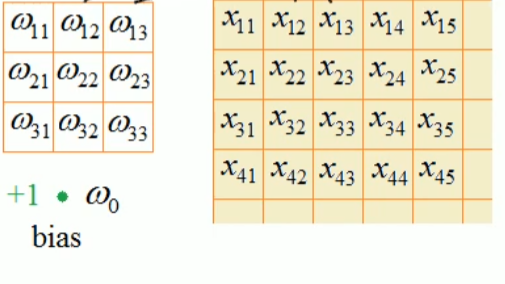
\includegraphics [scale=0.9] {img/conv.png}
  \caption{Пример ядра и часть матрицы входных данных} 
  \label{fig:2}  
\end{figure}

Элементы матриц ядер $w_{ij}$ и будут являться весами, которые необходимо определить в процессе обучения, они поэлементно умножаются на значения входных данных $x_{k,m}$:
\begin{equation}\label{eq:Vkm}
 v_{k,m} = \sum_{i=1}^{3}{\sum_{j=1}^{3}{x_{i+k,i+m}*w_{ij}}}+w_{0},
\end{equation}
где $k,m = 0,1,2,3...$

В конце каждой свертки на полученных данных $v_{k,m}$ используется выбранная на этапе проектирования функция активации для получения элементов карт признаков $O_{k,m}$:

\begin{equation}\label{eq:Okm}
O_{k,m}=f(v_{k,m}).
\end{equation}


Справедливо заметить, что в таком случае размерность карт признаков по обеим осям уменьшится на 2. Для избежания этой проблемы необходжимо добавить граничные значения, которые, как правило, нулевые (рисунок \ref{fig:3}).

\begin{figure}[ht] 
  \center
  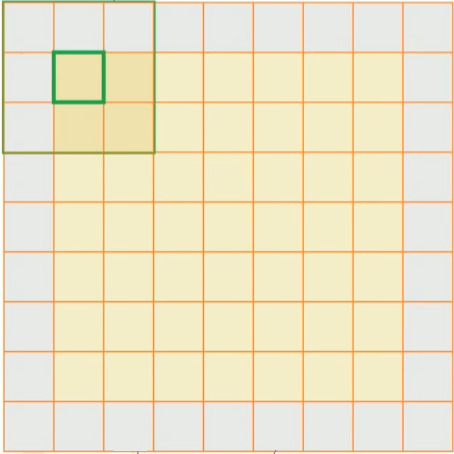
\includegraphics [scale=0.9] {img/padd.png}
  \caption{Пример добавлеия граничных значений} 
  \label{fig:3}  
\end{figure}

Также между сверточными слоями можно добавлять пулинг слои для уменьшения масштаба.

Второй частью является полносвязная нейронная сеть, на вход которой подается полученный вектор признаков.